%%%%%%%%%%%%%%%%%%%%%%%%%%%%%%%%%%%%%%%%%%%%%%%%%%%%%%%%%%%%%%%%%%%%%%%%%%%%%%%
%                       CARREGA DE LA CLASSE DE DOCUMENT                      %
%                                                                             %
% Les opcions admissibles son:                                                %
%      12pt / 11pt            (cos dels tipus de lletra; no feu servir 10pt)  %
%                                                                             %
% catalan/spanish/english     (llengua principal del treball)                 %
%                                                                             % 
% french/italian/german...    (si necessiteu fer servir alguna altra llengua) %
%                                                                             %
% listoffigures               (El document inclou un Index de figures)        %
% listoftables                (El document inclou un Index de taules)         %
% listofquadres               (El document inclou un Index de quadres)        %
% listofalgorithms            (El document inclou un Index d'algorismes)      %
%                                                                             %
%%%%%%%%%%%%%%%%%%%%%%%%%%%%%%%%%%%%%%%%%%%%%%%%%%%%%%%%%%%%%%%%%%%%%%%%%%%%%%%

\documentclass[11pt,spanish,listoffigures,listoftables]{tfgetsinf}

%%%%%%%%%%%%%%%%%%%%%%%%%%%%%%%%%%%%%%%%%%%%%%%%%%%%%%%%%%%%%%%%%%%%%%%%%%%%%%%
%                     CODIFICACIO DEL FITXER FONT                             %
%                                                                             %
%    windows fa servir normalment 'ansinew'                                   %
%    amb linux es possible que siga 'latin1' o 'latin9'                       %
%    Pero el mes recomanable es fer servir utf8 (unicode 8)                   %
%                                          (si el vostre editor ho permet)    % 
%%%%%%%%%%%%%%%%%%%%%%%%%%%%%%%%%%%%%%%%%%%%%%%%%%%%%%%%%%%%%%%%%%%%%%%%%%%%%%%

\usepackage[utf8]{inputenc} 

%%%%%%%%%%%%%%%%%%%%%%%%%%%%%%%%%%%%%%%%%%%%%%%%%%%%%%%%%%%%%%%%%%%%%%%%%%%%%%%
%                        ALTRES PAQUETS I DEFINICIONS                         %
%                                                                             %
% Carregueu aci els paquets que necessiteu i declareu les comandes i entorns  %
%                                          (aquesta seccio pot ser buida)     %
%%%%%%%%%%%%%%%%%%%%%%%%%%%%%%%%%%%%%%%%%%%%%%%%%%%%%%%%%%%%%%%%%%%%%%%%%%%%%%%



%%%%%%%%%%%%%%%%%%%%%%%%%%%%%%%%%%%%%%%%%%%%%%%%%%%%%%%%%%%%%%%%%%%%%%%%%%%%%%%
%                        DADES DEL TREBALL                                    %
%                                                                             %
% titol, alumne, tutor i curs academic                                        %
%%%%%%%%%%%%%%%%%%%%%%%%%%%%%%%%%%%%%%%%%%%%%%%%%%%%%%%%%%%%%%%%%%%%%%%%%%%%%%%

\title{Problema de regresión \\
         Resistencia a la compresión del hormigón}
\author{Luis Cabrero García}
\tutor{José María Valls Ferrán}
\curs{4º - Gr80}

%%%%%%%%%%%%%%%%%%%%%%%%%%%%%%%%%%%%%%%%%%%%%%%%%%%%%%%%%%%%%%%%%%%%%%%%%%%%%%%
%                              INICI DEL DOCUMENT                             %
%%%%%%%%%%%%%%%%%%%%%%%%%%%%%%%%%%%%%%%%%%%%%%%%%%%%%%%%%%%%%%%%%%%%%%%%%%%%%%%

\begin{document}

%%%%%%%%%%%%%%%%%%%%%%%%%%%%%%%%%%%%%%%%%%%%%%%%%%%%%%%%%%%%%%%%%%%%%%%%%%%%%%%
%              RESUMS DEL TFG EN VALENCIA, CASTELLA I ANGLES                  %
%%%%%%%%%%%%%%%%%%%%%%%%%%%%%%%%%%%%%%%%%%%%%%%%%%%%%%%%%%%%%%%%%%%%%%%%%%%%%%%

\makeindexes

%%%%%%%%%%%%%%%%%%%%%%%%%%%%%%%%%%%%%%%%%%%%%%%%%%%%%%%%%%%%%%%%%%%%%%%%%%%%%%%
%                              CONTINGUT DEL TREBALL                          %
%%%%%%%%%%%%%%%%%%%%%%%%%%%%%%%%%%%%%%%%%%%%%%%%%%%%%%%%%%%%%%%%%%%%%%%%%%%%%%%

\mainmatter

%%%%%%%%%%%%%%%%%%%%%%%%%%%%%%%%%%%%%%%%%%%%%%%%%%%%%%%%%%%%%%%%%%%%%%%%%%%%%%%
%                                  INTRODUCCIÓN                               %
%%%%%%%%%%%%%%%%%%%%%%%%%%%%%%%%%%%%%%%%%%%%%%%%%%%%%%%%%%%%%%%%%%%%%%%%%%%%%%%

\chapter{Introducci\'on}

\par La presente práctica trata de abordar mediante el punto de vista de las redes de neuronas supervisadas la resolución de un problema real: la predicción de la resistencia del hormigón a la fuerza de compresión. Para ello disponemos de ocho variables de entrada: la edad del hormigón en días y siete variables que representan los componentes que forman el hormigón (cemento, escoria de alto horno, cenizas volantes, agua, superplastificante, agregado grueso y agregado fino). Estos datos han sido tomados del KEEL\cite{KEEL}.

\section{Motivaci\'on}

\par La utilidad de los modelos de regresión que vamos a aplicar de forma práctica es reseñable: nos permiten determinar el valor de la resistencia a la compresión del hormigón a partir de sus características, lo que tiene bastante interés a la hora de saber predecir la resistencia del material en construcciones reales. Si somos capaces de mirar un poco más alla somos capaces de ver que estos modelos de regresión lineal (Adaline) y no lineal (Perceptrón multicapa) son capaces de estimar salidas en función de los datos de entrada pero no solo en este caso sino en problemas de otra índole. Esto nos da una primera idea de la potencia de estos modelos.

\section{Objetivos}

\par Los objetivos de la práctica son: procesar los datos del KEEL\cite{KEEL}, implementar el aprendizaje del modelo Adaline en el lenguaje de programación deseado (en mi caso PHP), grabar en distintos ficheros los resultados del aprendizaje de la red, las salidas obtenidas y error cometido para el conjunto de test, y posteriormente realizar experimentación con MLP y el modelo Adaline. Posteriormente se realizará una comparación entre ambos modelos para ver en que casos un modelo puede aproximar mejor que el otro.

\section{Estructura de la memoria}

\par La memoria dispone de tres índices, uno para consultar cada una de las secciones y otros dos para figuras y tablas. En la memoria se puede encontrar un apartado general para el modelo Adaline y otro para el Perceptrón multicapa. Dentro de los respectivos apartados de cada modelo, se explica la base teórica de cada uno de ellos, se explica la implementación en el caso de Adaline, y en ambos se explica los distintos experimentos realizados y se razona el motivo por el que se consideran dichos experimentos como necesarios y suficientes. En las conclusiones se explican las diferencias entre ambos modelos y se comparan los resultados obtenidos en la experimentación. Al final de la memoria se indican las referencias bibliográficas consultadas para llevar a cabo el siguiente trabajo.

%\section{Notes bibliografiques} %%%%% Opcional

%????? ????????????? ????????????? ????????????? ????????????? ?????????????

%%%%%%%%%%%%%%%%%%%%%%%%%%%%%%%%%%%%%%%%%%%%%%%%%%%%%%%%%%%%%%%%%%%%%%%%%%%%%%%
%                         CAPITOLS (tants com calga)                          %
%%%%%%%%%%%%%%%%%%%%%%%%%%%%%%%%%%%%%%%%%%%%%%%%%%%%%%%%%%%%%%%%%%%%%%%%%%%%%%%

\chapter{Modelo Adaline}

\par En este capítulo se va a explicar en primer lugar el modelo Adaline, se va a indicar cuales son sus ventajas e inconvenientes, se explicará la implementación que se ha llevado a cabo en PHP y el formato que se ha elegido para devolver las salidas del modelo. También se expermientará con distintos ciclos de aprendizaje y distintas razones de aprendizaje, y se verá el comportamiento de la red en todos los casos posibles, para ello se representará cada posible situación con un experimento para abordar todos los casos posibles.

\section{ADALINE: ADAptive LInear NEuron}

\par Es un tipo de red de neuronas artificiales desarrollada por Bernard Widrow y Ted Hoff. La red está compuesta por \textit{n} neuronas(\ref{fig:adaline}), con \textit{m} entradas. La salida de cada neurona se representa por la función de activación(\ref{eq:ej}) y representa el impacto de cada peso sobre las entradas, sumando el umbral de la neurona (\theta).

\begin{equation}\label{eq:ej}
y = \sum_{i=1}^{n}w_{i}*x_{i} + \theta
\end{equation}

\begin{figure}
\centering
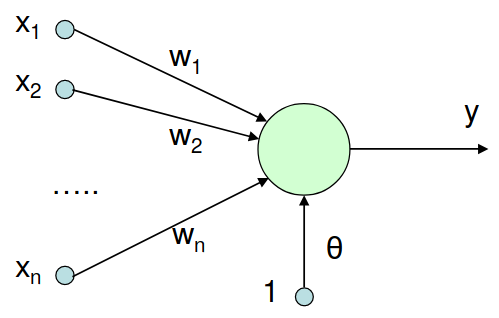
\includegraphics[scale=0.5]{adaline}
\caption{Neurona ADALINE \cite{Adaline}}\label{fig:adaline}
\end{figure}

\par En el caso que nos ocupa(\ref{eq:ej2}), teniendo ocho entradas, la salida que se obtiene es la estimación de la resistencia del hormigón a la compresión. Los pesos aplicables a cada una de las entradas, junto con el umbral, se inicializan de manera aleatoria entre \textit{-0.5} y \textit{0.5}.

\begin{equation}\label{eq:ej2}
ConcreteCompressiveStrengthEst = \sum_{i=1}^{8}w_{i}*x_{i} + \theta
\end{equation}

\par El \textbf{aprendizaje} de la red, se realiza teniendo en cuenta la diferencia entre la salida deseada (adjunta como dato en los conjuntos de entrenamiento, test y validación) y la salida obtenida(\ref{eq:ej}). Teniendo en cuenta esta diferencia se trata de minimizar el error obtenido mediante la modificación de los pesos y el umbral. Para hallar el error cuadrático medio(\ref{eq:ej3}) se opera con todos los errores cuadráticos obtenidos en cada uno de los \textit{N} patrones. 

\begin{equation}\label{eq:ej3}
E = \frac{1}{N}* \sum_{p=1}^{N}(d^{p} - y^{p})^{2}
\end{equation}

\par Por último, la modificación de los pesos y umbral se realiza siguiendo la Regla Delta, que busca la minimización iterativa de la función de error(\ref{eq:ej3}), realizando un cambio a cada peso proporcional a la derivada del error, medida en el patrón actual, respecto del peso (\ref{eq:ej4}). El umbral también se modifica(\ref{eq:ej5}).

\begin{equation}\label{eq:ej4}
\Delta_{p}w_{j} = -\gamma\frac{\partial E^{p}}{\partial w_{j}} = \gamma*(d^{p} - y^{p})*x_{j}
\end{equation} 

\begin{equation}\label{eq:ej5}
\Delta_{p}\theta = \gamma*(d^{p} - y^{p})
\end{equation}

\par siendo $\gamma$ la razón o tasa de aprendizaje.

\par En este punto es importante resaltar que los datos deben \textbf{normalizarse}, \textbf{aleatorizarse} y \textbf{separados} en tres conjuntos de datos: \textbf{entrenamiento}, \textbf{validación} y \textbf{test}.

\begin{itemize}
\item \textbf{Datos de entrenamiento}: (70\%  del  total  de  datos) para  realizar  el aprendizaje de la red. 
\item \textbf{Datos de validación}: (15\%  del  total  de  datos) utilizados para elegir los  valores  óptimos  de los parámetros  de  la  red  (razón  de aprendizaje, número de ciclos, número de neuronas).
\item \textbf{Datos de test}: (15\%  del  total  de  datos) para evaluar la capacidad de generalización de la red.
\end{itemize}

\section{Implementación del modelo}

\par El modelo se ha decidido implementar en PHP por estar el autor familiarizado con dicho lenguaje y por la tremenda facilidad que ofrece a la hora de hacer cambios de tipo. En el fichero adaline.php se define la clase Adaline, que tiene atributos que caracterizan a la red de una sola neurona. Se leen los parámetros pasados por terminal y se ejecuta el aprendizaje de la red. Posteriormente se pasa el conjunto de validación y por último se pasa el conjunto de test.

\begin{lstlisting}
<?php

   //EJECUCION: php entrenamiento.php <tasa_aprendizaje> <num_ciclos>

   include 'adaline.php';
   $tasa_aprendizaje = $argv[1];
   $num_ciclos = $argv[2];
   $adaline = new Adaline($tasa_aprendizaje);
   $adaline->ejecutaradaline($num_ciclos);

?>
\end{lstlisting}

\par \textbf{Especificación de los métodos implementados}

\begin{itemize}
\item \textit{construct}. Parámetro: tasa de aprendizaje. Inicializa pesos y umbral de manera aleatoria, inicializa la tasa de aprendizaje, inicializa los arrays necesarios.
\item \textit{aprendizaje}. Parámetros: fichero a utilizar y ciclo. Realiza el aprendizaje de la red utilizando los datos de entrenamiento provenientes de un fichero csv.
\item \textit{error}. Parámetros: fichero a utilizar y ciclo. Calcula el error producido en un ciclo de entrenamiento sin modificar los pesos ni el umbral.
\item \textit{errorvalidacion}. Parámetros: fichero a utilizar y ciclo. Calcula el error producido en un ciclo de validación sin modificar los pesos ni el umbral.
\item \textit{errortest}. Parámetro: fichero a utilizar. Calcula el error cuadrático medio sobre el conjunto de los datos de test.
\item \textit{resultados}. Parámetros: carpeta, ciclo y número de ciclos. Muestra en un fichero HTML las salidas obtenidas para el conjunto de entrenamiento y validación normalizadas y desnormalizadas.
\item \textit{mostrarerrores}. Parámetros: carpeta y número de ciclos. Muestra en un fichero HTML los errores cuadráticos medios por cada ciclo para entrenamiento y validación, el valor del error cuadrático medio para el conjunto de test, los pesos y umbral resultantes tras aprendizaje y las salidas desnormalizadas de test.
\item \textit{datostest}. Parámetros: carpeta y número de ciclos. Muestra en un fichero HTML los errores sobre el conjunto de test normalizado y sin normalizar, muestra también una gráfica comparando las salidas obtenidas con las esperadas.
\end{itemize}

\section{Experimentación realizada}

\par La experimentación realizada en Adaline se basa en ir variando la razón de aprendizaje ($\gamma$) y el número de ciclos de ejecución. Iremos extrayendo ciertas conclusiones en función de los valores posibles de $\gamma$, entre 0 y 1 y los ciclos de ejecución, que pueden ser desde 1 al número que se quiera indicar.

\par \underline{\textbf{Experimentaciones}}

\par \textbf{$\gamma = 0.8$ y $ciclos = 500$}

\par Con una tasa de 0.8 y 500 ciclos la red "no aprende" (\ref{fig:8500}) dado que comienza cometiendo un error y en el ciclo inmediatamente posterior el error aumenta, tendencia que continúa hasta que el error se estabiliza en un valor elevado, por tanto considero de poco interés este experimento. El error obtenido sobre el conjunto de test es de 0.49219936325144.

\begin{figure}[H]
\centering
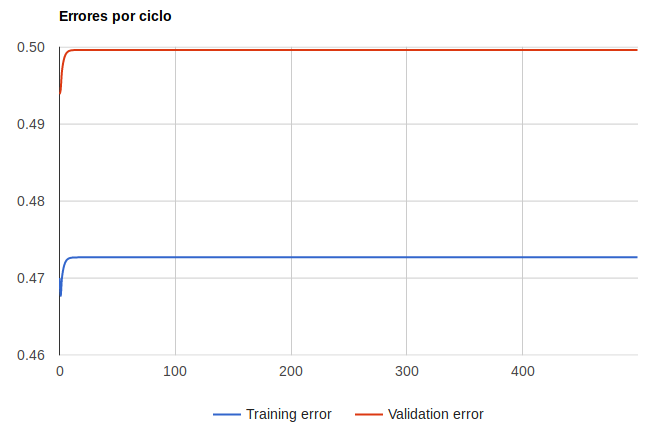
\includegraphics[scale=0.5]{8500}
\caption{Gráfica Adaline 0.8 - 500}\label{fig:8500}
\end{figure}

\par \textbf{$\gamma = 0.2$ y $ciclos = 500$}

\par Con una tasa de 0.2 y 500 ciclos (\ref{fig:2500}) se produce un claro sobreaprendizaje dado que la red es capaz de generalizar el conjunto de entrenamiento con un error cuadrático medio que se estabiliza en torno a 0.021043565092019 mientras que el conjunto de validación se estabiliza en torno a 0.021394445575013. Como vemos la diferencia es muy pequeña pero digamos que en este valor se comienza a producir el sobreaprendizaje, situación que no deseamos porque esto indica que la red no será capaz de generalizar bien datos que no conozca. El error de test es de 0.023142903383433.

\begin{figure}[H]
\centering
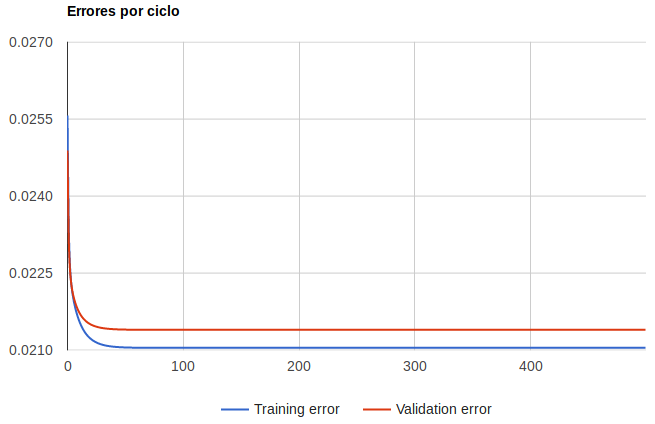
\includegraphics[scale=0.5]{2500}
\caption{Gráfica Adaline 0.2 - 500}\label{fig:2500}
\end{figure}

\par \textbf{$\gamma = 0.15$ y $ciclos = 500$, $\gamma = 0.1$ y $ciclos = 500$}

\par Con una tasa de 0.15 y 500 ciclos se sigue produciendo sobreaprendizaje pero se puede observar que según se va disminuyendo la tasa de aprendizaje, el valor absoluto de la diferencia entre ambos errores va disminuyendo. También va disminuyendo el error de test que ahora se sitúa en 0.021433296435724. Esta tendencia se puede comprobar con la experimentación realizada para $\gamma = 0.1$ y $ciclos = 500$ (\ref{fig:1500}). El error de entrenamiento se estabiliza en 0.017396882217266 y el de validación en 0.018214407942476. El error producido en test en este caso es de 0.020000915138424. En este caso, con $\gamma = 0.1$ sigue produciendose sobreaprendizaje.

\begin{figure}[H]
\centering
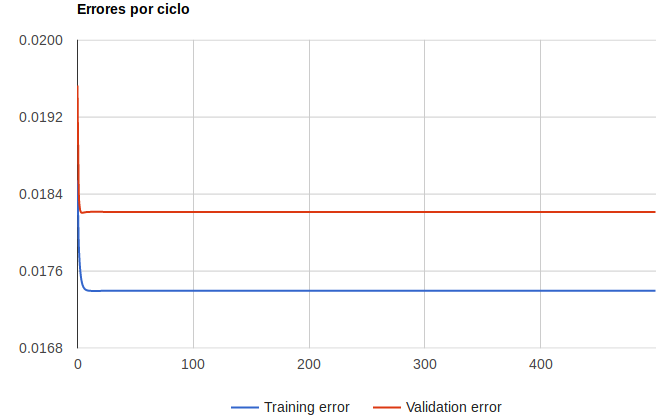
\includegraphics[scale=0.5]{1500}
\caption{Gráfica Adaline 0.1 - 500}\label{fig:1500}
\end{figure}

\par \textbf{$\gamma = 0.0001$ y $ciclos = 20000$}

\par Con una tasa muy pequeña ($\gamma = 0.0001$) son necesarios cerca de 20000 ciclos (\ref{fig:000120000}) para conseguir que los errores de validación y entrenamiento se estabilicen. Se obtienen 0.016186448864616 y 0.016999895299418 como errores estabilizados en entrenamiento y validación respectivamente. El error producido sobre el conjunto de test es 0.019147481314295.

\begin{figure}[H]
\centering
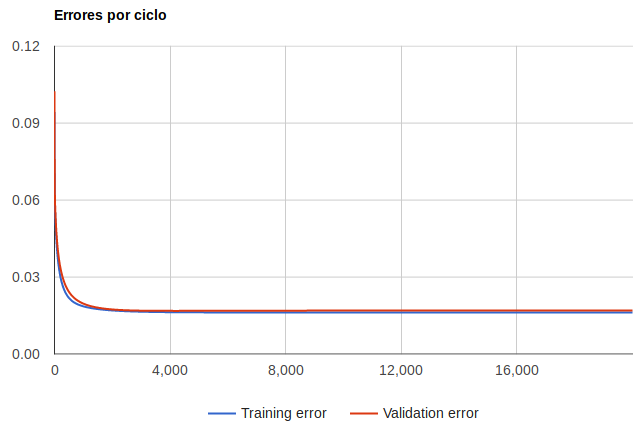
\includegraphics[scale=0.5]{000120000}
\caption{Gráfica Adaline 0.0001 - 20000}\label{fig:000120000}
\end{figure}

\section{Resumen experimentación Adaline}

\begin{table}[H]
\centering
\caption{Resumen experimentación Adaline}
\label{tb:tb1}
\begin{tabular}{lllll}
\hline
\multicolumn{1}{|l|}{Tasa de aprendizaje} & Error entrenamiento & Error validación  & Error test        \\ \hline \hline
0.8                                       & 0.47269316589935    & 0.49962652341666  & 0.49219936325144  \\
0.2                                       & 0.021043565092019   & 0.021394445575013 & 0.023142903383433 \\
0.1                                       & 0.017396882217266   & 0.018214407942476 & 0.020000915138424 \\
0.0001                                    & 0.016186448864616   & 0.016999895299418 & 0.019147481314295 \\ \hline
\end{tabular}
\end{table}

\begin{figure}[H]
\centering
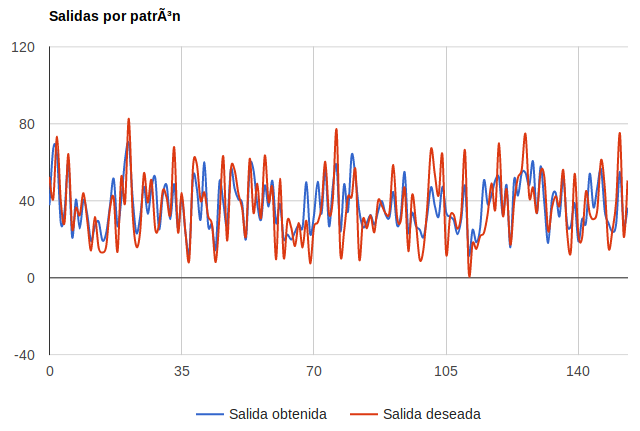
\includegraphics[scale=0.5]{bestadaline}
\caption{Salidas obtenidas vs salidas deseadas para tasa de aprendizaje 0.0001}\label{fig:bestadaline}
\end{figure}

\par Como vemos, el mejor experimento realizado es aquel que minimiza el error cuadrático medio, esto es, el realizado con tasa de aprendizaje 0.0001, por lo que se muestran las salidas obtenidas frente a las deseadas en dicho experimento. Podemos ver que para algunas de las salidas el modelo aproxima casi a la perfección pero para otras hay grandes diferencias, en esas diferencias es en las que se genera el error que en este caso se eleva a 123.26694496161, valor desnormalizado. Posteriormente evaluaremos el MLP y veremos si estos valores son mejorables \footnote{Para ver los valores en detalle acudir a los resultados adjuntos en formato HTML}.

\chapter{Modelo Perceptrón Multicapa}

????? ????????????? ????????????? ????????????? ????????????? ????????????? 

\section{Perceptron Multicapa (MLP)}

????? ???????El objetivo es obtener una red tal que y?????? ????????????? ????????????? ????????????? ?????????????

\section{Experimentación realizada}

%%%%%%%%%%%%%%%%%%%%%%%%%%%%%%%%%%%%%%%%%%%%%%%%%%%%%%%%%%%%%%%%%%%%%%%%%%%%%%%
%                                 CONCLUSIONS                                 %
%%%%%%%%%%%%%%%%%%%%%%%%%%%%%%%%%%%%%%%%%%%%%%%%%%%%%%%%%%%%%%%%%%%%%%%%%%%%%%%

\chapter{Conclusiones}

Hablar del tema rendimiento
Comparar ambos modelos

????? ????????????? ????????????? ????????????? ????????????? ????????????? 

%%%%%%%%%%%%%%%%%%%%%%%%%%%%%%%%%%%%%%%%%%%%%%%%%%%%%%%%%%%%%%%%%%%%%%%%%%%%%%%
%                                BIBLIOGRAFIA                                 %
%%%%%%%%%%%%%%%%%%%%%%%%%%%%%%%%%%%%%%%%%%%%%%%%%%%%%%%%%%%%%%%%%%%%%%%%%%%%%%%

\begin{thebibliography}{10}


\bibitem{KEEL}
   Conjunto de datos del hormigón, 
   \newblock Knowledge Extraction based on Evolutionary Learning. 
   \newblock Obtenido de
   \url{http://sci2s.ugr.es/keel/dataset.php?cod=44}.

\bibitem{Adaline}
   Primeros modelos computacionales, 
   \newblock Inés M. Galván y José Mª Valls.
   \newblock Obtenido de
   \url{http://ocw.uc3m.es/ingenieria-informatica/redes-de-neuronas-artificiales/transparencias/material-de-clase.-tema-2/view}.

\bibitem{MLP}
   Peceptrón Multicapa, 
   \newblock Inés M. Galván y José Mª Valls.
   \newblock Obtenido de
   \url{http://ocw.uc3m.es/ingenieria-informatica/redes-de-neuronas-artificiales/transparencias/material-de-clase.-tema-3/view}.

\end{thebibliography}
\cleardoublepage

%%%%%%%%%%%%%%%%%%%%%%%%%%%%%%%%%%%%%%%%%%%%%%%%%%%%%%%%%%%%%%%%%%%%%%%%%%%%%%%
%                              FI DEL DOCUMENT                                %
%%%%%%%%%%%%%%%%%%%%%%%%%%%%%%%%%%%%%%%%%%%%%%%%%%%%%%%%%%%%%%%%%%%%%%%%%%%%%%%

\end{document}
